
\chapter{Implementation of segmentation, ABCD rules  and Dermoscopic structures}

\section{Introduction}
This chapter is a discussion of the most popular ABCD (Asymmetry, Border, Colour, and Dermoscopic Features) algorithms including their implementation, and updating the algorithms. They are compared using the PH2 dataset and updated relating to their accuracy. Surprisingly, many of the ABCD rules techniques were originally tested for whether they effectively find melanoma and not individual features. So, this will be the first time some of these techniques were tested and documented.

%Discuss the ABCD rule techniques and how border is better with a tighter border rather than segmentation from techniques including SegNet

\section{Hybrid Melanoma Segmentation Algorithms using Neural Networks and Statistical Models}
Segmentation plays a crucial role in melanoma detection because it separates melanoma from healthy skin. Accurate segmentation is essential for various aspects of melanoma diagnosis, treatment, and classification\cite{Albahli2020} including improving the detection of ABCD rules\cite{Lee2020}. This is especially important for border analysis\cite{Pereira2020, Kaya2016} that relies on the analysis of convex and indents. The irregularity of borders is a key feature in distinguishing melanoma from benign lesions, and exact identification of irregular borders from melanoma skin lesions is clinically significant\cite{patil2021}.

There are various deep learning approaches\cite{Albahli2020} and deep CNN techniques\cite{yu2017}. These highlight the significance of advanced technologies for accurate segmentation and detection of melanoma. Although these techniques are massively accurate they are trained using datasets (ISIC 2019) contain rough segmentation masks, resulting in the produced borders having a poor border cut-off. This can be seen further in figure\ref{seg-expert}. This is largely due to ISIC datasets only having a few expert borders and not enough to train deep learning algorithms. Furthermore, the images are also shrunk as part of the deep learning process, which in turn loses smaller features that are of significant when analysing borders. All of this results in the major technologies including deep learning are ineffective when producing border cut-off.

%Show example of borders and expert borders
\begin{figure}[]
    \centering
    %\includegraphics[scale=1.2]{images/}
    \caption{Some images from the ISIC dataset demonstrating the difference between segmentation masks and expert segmentation masks.}\label{seg-expert}
\end{figure}

A range of traditional segmentation techniques including SegNet, U-net methods have been shown to outperform other approaches in capturing the most significant melanoma characteristics. However, these techniques do not provide an effective border for the analysis of ABCD rules. Various statistical algorithms have been explored including active contouring-based segmenatation\cite{Riaz2019}, LBPC and others for border adjustment including u-otsu and edge-imfill.

\subsection{Related Works}
An approach by Albanhli\cite{Albahli2020} uses a deep learning-based segmentation algorithm using YOLOv4-DarkNet and active contouring for melanoma and skin lesion detection and segmentation. This technique provides a classification of the skin lesion and a segmentation, demonstrating a high level of practicality for clinical decision support systems. 

Seeja R D\cite{seeja2019} proposed a technique that utilizes a convolutional neural network (CNN) based on a U-net model architecture for the segmentation based on colour, texture, and shapes. The U-net model architecture is a popular choice for image segmentation tasks due to its ability to capture both local and global features effectively.

Hyunju Lee\cite{Lee2020} proposed a technique that utilizes an edge fill method called u-otsu for segmentation, using the U channel from the YUV colour space to calculate the histogram. Otsu calculates the optimal threshold value to separate foreground and background pixels based on the histogram of the image.

Another technique by Pedro\cite{Pereira2020} uses a newly developed technique called Local Binary Patterns Clustering (LBPC). Using a Local Binary Pattern (LBP) filter by subtracting the gray-scale image from the LBP filter after a Gaussian filter, resulting in the creation of a mask. This has been successfully used for the detection of melanoma.

\subsection{Semantic Pixel Wise Segmentation (SegNet)}
Semantic pixel-wise segmentation (SegNet) is a deep learning architecture that is used for semantic image segmentation for melanoma detection. It was originally developed by\cite{chen2018} and has shown promising results in various segmentation tasks. The idea of SegNet is to perform pixel-wise classification by assigning each pixel in an image to a specific class or category. This is achieved through a fully convolutional neural network (FCN) architecture, which allows for end-to-end learning and inference at the pixel level. 

Semantic pixel-wise segmentation (SegNet) is a machine learning architecture utilizing a deep, fully convolutional neural network (DCNN). This network requires training from ground truth and pre-segmented images for automatic segmentation. SegNet consists of encoding layers, decoding layers, and a pixel-wise classification layer. The encoder layers consist of 3$\times$3 convolutions (including batch normalization and ReLU), and pre-trained filters for classifying features. After some convolutions, the data is down-sampled using a 2$\times$2 pooling layer. Next, decoding layers consist of up-sampling, followed by 3$\times$3 convolutions. Finally, the pixel-wise classification uses a softmax layer to represent each pixel between 0 and 1 based on the previous layers, generating a segmentation mask.

\begin{figure}[hb]
\centering
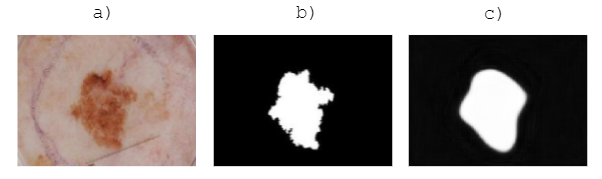
\includegraphics[scale=1.2]{images/border-seg.png}
\caption{Demonstrating the Semantic Pixel-Wise Segmentation (SegNet) results showing the a) original image, b) expert ground-truth and c) SegNet results.}\label{SegNet}
\end{figure}



Results in figure \ref{SegNet} are generated from the architecture using the ISIC 2018 dataset split into 80\% training and 20\% validation images. The accuracy of locating the lesions is 85\%. However, figure \ref{SegNet} represents the border cut-off between skin and skin lesion is accurate to the dataset but inadequate for using the ABCD rules. Finding the border cut-off is vital for measuring ABCD rules\cite{Pereira2020}.

\subsection{U-Otsu Threshold}
Otsu threshold is a versatile automatic image thresholding technique meant to separate each pixel between two classes of foreground or background. One of the benefits of this method is that it does not require any training data. The equation \ref{otsu} (within-class variance) describes splitting weights of $w_0(t),w_1(t)$, which are the probabilities divided by the threshold $t$, between 0 and 255. Furthermore, $\sigma_1^2$ and $\sigma_0^2$ are variances of these two classes. The class probability $w$ is computed from the histogram in figure \ref{otsu2}, which is an intensity histogram describing the colour distribution in an image. Measuring the values above and below the generated thresholds splits the image into two classes.

\begin{equation}
\sigma_w^2(t) = w_0(t)\sigma_1^2(t) + w_1(t)\sigma_2^2(t)
\end{equation}\label{otsu}

The histogram was split into two segments with the threshold $t$ of 138 and the corresponding pixel locations to the histogram segment the skin lesion into two classes. Image morphology closing was applied to fill gaps that the threshold missed. On other occasions, the segmentation missed the skin lesion because of a similar colour between the skin and the skin lesion. It might be beneficial to combine Otsu with SegNet to improve its accuracy while producing a border cut-off. Figure \ref{otsu2} describes the difference between otsu and SegNet.

\begin{figure}
\centering
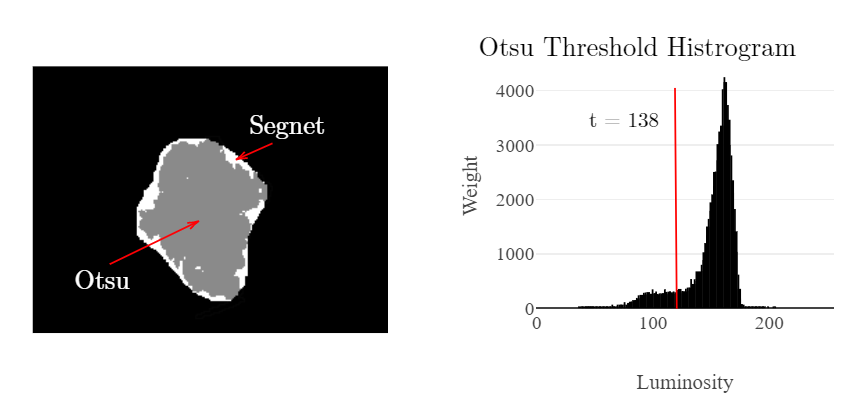
\includegraphics[scale=0.7]{images/otsu3.png}
\caption{Otsu thresholding alongside ground-truth mask, where grey Otsu and white is SegNet. The bar chart shows the histogram with an otsu threshold of 138.}\label{otsu2}
\end{figure}


\subsection{LBPC segmentation}
Local Binary Patterns (LBP) is a texture descriptor commonly used for augmenting the image improving classification accuracy\cite{Pereira2020, Kaya2016}. First, equation\ref{eq1} calculates each pixel, where $p$ (equal to 8) is the number of neighbouring pixels compared to the centre of $c$, and the radius of $r$ from the centre. Next, shown in equation\ref{eq2} each value is subtracted counter-clockwise with the centre value and compared to function $S$ where each $gp - gc$, if more than or equal to 0, is equal to 1, and less than 0 is equal to 0. Next, add corresponding values equal to 1 of $gp$ together, changing the centre value, ignoring values of 0. Next, applying a Gaussian kernel of 13-pixel iterations and a standard deviation of 3 removes smaller features that interfere with the segmentation. Finally, applying k-means with a value of 2 subtracts the greyscale and segments the skin lesion from the skin.

\begin{equation} \label{eq1}
LBP(gp_x, gp_y) = \mathlarger{\sum}_{p=0}^{P-1}s\big(gp - gc)2^p
\end{equation}

\begin{equation} \label{eq2}
s\big(x) = 
\begin{cases}
1,\:\:x\geq\:0; \\
0,\:$otherwise$.
\end{cases}
\end{equation}

Figure \ref{fractal1} demonstrates the segmentation of two skin lesions, one with an irregular border and another with a regular border. LBPC is applied to both skin lesions, followed by Gaussian blurring and morphology closing to remove dots. The result is an improved border cut-off compared to the ground truth in the Ph$^2$ dataset with more corners and ledges. This technique will improve accuracy for measuring border irregularity\cite{Pereira2020}.

\begin{figure}
\centering
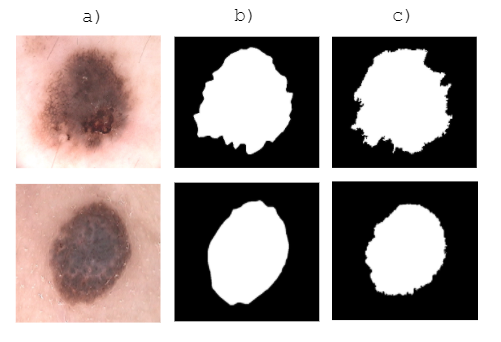
\includegraphics[scale=1.2]{images/borders.PNG}
\caption{Local Binary Pattern Clustering (LBPC) showing the a) original image, b) ground-truth, and c) LBPC. LBPC successfully exaggerates the border cut-off on the skin lesions with regular and irregular borders} 
\end{figure}\label{fractal1}

Validating LBPC is not expected because the goal is to exaggerate the border to improve the classification process of ABCD rules, which it does successfully\cite{Pereira2020, Kaya2016}. For example, the segmentation might not match dataset segmentations but is still essential to classifying ABCD rules. Furthermore, many datasets lack expert border segmentation, an accurate border cut-off between the skin and skin lesions, so comparisons are not always possible.

\subsection{Results}
Overall the accuracy of the techniques demonstrates that SegNet is the most reliable technique. However, comparing the techniques in \ref{} we can demonstrate that it produces a smudge effect and fails to capture the border cut-off from the skin lesion, but it is successful at finding the location of the skin lesion.

Both statistical models of LBPC and Otsu threshold generated an accurate border cut-off between the skin and the skin lesion As previously mentioned, measuring the border cut-off and exaggerating irregular borders are helpful when calculating the ABCD rules. 

It might be beneficial to combine SegNet and LBPC using SegNet to find the skin lesions' location, followed by adjusting the border cut-off using LBPC. A similar technique using the Otsu threshold and Segnet is described by Riaz et al.\cite{Riaz2019}.

%Tables showing the accuracy of all three of the techniques essentially showing that segnet is obviously better.

\subsubsection{Border Cut-off}
%Show that regardless of segnet being better that the other techniques still have a better border cut-off improving border irregulrity detection
This section includes a simple border analysis technique called fractal box counting to assess the benefits of using different segmentation algorithms with accurate border cut-offs.

To prove the usefulness of segmentation techniques with an accurate border cut-off a technique developed by Ali\cite{Ali2020b} is implemented that utilises machine learning with extracted data including Zernike moments, fractal box-counting, and convexity measurements. Fractal box-counting is used to measure the irregularity of the border.

The fractal box-counting technique is a commonly employed technique for analysing fractal properties. It involves dividing a fractal object or pattern into a grid of equally sized boxes and counting the number of boxes that contain a portion of the fractals. The process is repeated with different box sizes until the boxes until the relationship between the box sizes and number of boxes is analysed determining the fractal dimension\cite{Hamburger1996}. Essentially a more complicated border with corners and convexes will have more boxes and therefore a higher fractal score, than for example a border with smooth corners and edges which has a lower score. This should provide some evidence of the usefulness of an accurate border.

\subsection{Issues}
%Show that LBPC sometimes fails at finding the skin lesion
The segmentation algorithms encountered some issues, whilst the best of the techniques was SegNet with an 85\% accuracy when relating to the ISIC 2019 dataset. However, as previously mentioned the segmentation masks have poor border cut-off stunting features that are useful for finding border irregularities. 

In contrast LBPC and U-Otsu algorithms effectively identify the border cut-off of the skin lesion, which isn't properly represented in the ISIC 2019 dataset. But, it sometimes fails to find the skin lesion or not detect anything. 

Both techniques appear to have downfalls making them less effective for use for analysing ABCD rules. It would be beneficial to find the approximate area of the skin lesion using SegNet and followed by LBPC to find the border cut-off.

\section{Joint Neural network and statistical model approach}
%Combine techniques together to get the area of the border
Combining both SegNet and LBPC improves the accuracy.

\section{ABCD Rules Data Extraction Techniques}
Melanoma is a type of malignant skin cancer that accounts for a significant proportion of cancer-related deaths around the world. In 2018 there were approximately 2,353 per 100,000 deaths in the United Kingdom (UK)\cite{UK2019}. Early detection is critical for improving the diagnosis and survival of patients. However, existing approaches including clinical examinations and dermoscopy, have limitations in terms of accuracy and cost-effectiveness\cite{Takiddin2021}. Machine learning approaches have beaten dermatologists in terms of accuracy\cite{Andre2017}. However, these approaches lack explainability implementing such techniques difficult for clinical environments\cite{Fan2017}. One concern is the production of realistic, but incorrect results\cite{Ghorbani2019}. Another is the use of parallel processes, which describes the creation of an answer with little to no explanation. In this paper, we propose a combined asymmetry approach using shape, colour, and texture analysis alongside a detailed comparison. The technique itself can be used in conjunction with ABCD rules (Asymmetry, border, colour, and dermoscopic features).

%Consider adding segmentation to this chapter, explain why its important for border irregualrity analysis

\subsection{Preferred Diagnostic Procedures}
% Quick summary of TDS, ABCD rules, bi-fold and general issues
Diagnostic procedures are procedures that are performed on patients in order to diagnose conditions. Regarding the diagnosis of melanoma, many types have been utilised for the detection of melanoma and the most favourable are CASH, ABCD rules, and Total Dermoscopy Score (TDS). The ABCD rules and TDS were commonly used because of their simplicity and effectiveness.

Diagnostic procedures are usually based on the doctors medical experience. For example the use-case of this project is for general practioners (GPs), many of which have likely never seen or attempted to diagnose melanoma, and many of which will not have access to dermoscopes for the analysis of dermoscopic structures. So, in this use-case diagnostic procedures including ABCD rules, and CASH are suitable because of their simplicity. The method used by the NHS is also ABCD rules, which is the reasoning for using this method. 

Interestingly dermatologists will utilise dermoscopic features and textures, which are more accurate but require sufficient training for the detection.

\subsubsection{Asymmetry Techniques}
Asymmetry analysis is a fundamental component in the early detection of melanoma because it often exhibits asymmetric shapes\cite{Ali2020a}. Meaning that the shape, colour and, texture match asymmetrically more often in benign lesions. For example, as melanoma grows the central area begins to waste away leaving a hollow area covered by thin skin, showing dermoscopic features. As it grows the edges become more irregular producing an uneven shape often relating to irregular borders and asymmetrical shapes. Diagnostic procedures have been developed to detect these unique characteristics.

Bi-fold is a diagnostic procedure designed to support the recognition of melanoma by drawing a line down the middle of the skin lesion and comparing the two halves to confirm whether the sides match (considering the difference in shape, colour, and texture). Using this horizontally and vertically calculates whether the skin lesion is possibly malignant with a score between 0 and 2. Calculating with Total Dermoscopy Score (TDS) alongside the other ABCD rules including asymmetry, border, colour, and diameter calculates the likelihood of malignancy. Dermatologists frequently use bi-fold due to its simplicity, but it can be subjective to the original observer and time-consuming when managing large numbers of skin lesions. Therefore, automating techniques is beneficial to clinicians and can improve the objectivity of results.

\subsection{Related Works}
% Measuring asymmetry shape
Ihab S. Zaqout\cite{Zaqout2016} describes a technique using the centroid and rotation of the skin lesion using moments of inertia. By Folding the skin lesion on both vertical and horizontal axes subtracting the opposite half. Pixels that cannot subtract are summed and compared with a threshold considering the skin lesion asymmetrical if the combined sum is more than the threshold.

% Measuring asymmetry colour
Kasmi and Mokrani\cite{Kasmi2016} create a grid of 20 by 20 pixels from the skin lesion image and convert it into the LAB colour space. They then compare the average colour of each block with a perpendicular block (vertical and horizontal axes) using the three-dimensional Euclidean luminance distance, a-axis, and b-axis. If more than half of the colour comparisons exceed the threshold, they consider that axis to be colour asymmetrical. They ignore blocks that have no symmetrical pair. Finally, they calculate luminance separately to prevent brightness problems. This technique achieves an accuracy of 94\% with a private dataset.

% Measuring asymmetry texture
Ali\cite{Ali2020a} uses SIFT-based similarity and projection profiles to measure similarities in texture. SIFT is scale-invariant and helpful for texture components with varying texture quality. First, they split the skin lesion vertically and horizontally across the centre into four halves, compare texture components on the symmetrical halves, and measure similarity. Lastly, they generate histograms for the projection profile in the x and y directions. These results train a decision tree and achieve an 80\% accuracy of the ISIC 2018 with 204 images privately annotated for ABCD rules.

% Summary of techniques and mention of the proposed approach
Prior studies have introduced techniques that measure distinct aspects of asymmetry, such as Ihab S. Zaqout\cite{Zaqout2016} measurement of shape, Kasmi and Mokrani\cite{Kasmi2016} measurement of colour, and  Ali\cite{Ali2020a} measurement of texture. The new approach seeks to combine the following approaches into a more comprehensive analysis of asymmetry that takes into account multiple features of the skin lesion. The proposed novel technique updates colour measurement to improve accuracy using superpixels and an SVM model.

\section{A Novel Asymmetry detection technique using Bi-Fold, 3D Euclidean distance, and Superpixels}
This section describes a novel machine-learning technique for the automatic detection of melanoma

\subsection{Bi-fold}
To initiate the classification of skin lesions a technique called bi-fold is applied involving folding the skin lesion in half vertically and horizontally and a comparison of their respective dimensions. While the original technique was designed only to assess the lesions' shape, it's been utilized to account for colour and texture as well. The centre and orientation are determined by calculating its moments, where the centre is (m10 / m00, m01 / m00) and phi is 0.5tan (2m11)/ (m20 -m02).

%Add diagram demonstrating bi-fold of a skin lesion

\subsection{3D Euclidean Distance}
Next, the lesion is partitioned into a 20 by 20 grid centred on the mentioned centre point, and the average of each region is computed. This is followed by finding the matching region on the perpendicular area from the centre of the skin lesion and comparing the colour distance between the two. Distance is measured using the LAB colour space and a 2D Euclidean distance of A and B, removing L (luminosity) to eliminate light variation. Once compared, all compared regions are obtained, and they are plotted onto a graph. If over half of the values are above a threshold of 6, then the lesion is asymmetrical.

% Scrutinize the threshold method and show the graph that the data can't be split with only the threshold 
The diagram shown below in figure\ref{symmetrical} is a compilation of all the images within the PH\^2 dataset showing the threshold range after applying bi-fold, euclidean distance of colour, but before applying the threshold. As can be seen, a threshold of 6 covers all of the symmetrical values, but still roughly covers half of the asymmetrical values. This demonstrates that the technique produces many false positives when regarding asymmetrical values.
Essentially, the symmetrical skin lesion has a smaller area and the asymmetrical lesion has a larger area, but both remain in the same zone and therefore splitting the data only using a threshold holds poor results. Furthermore, there are a lot of fliers and the threshold does not adjust according to these values. See the graph below:

\begin{figure} 
    \centering
    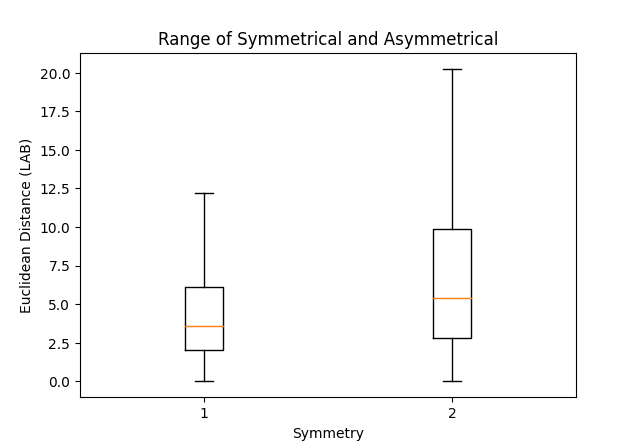
\includegraphics[scale=0.6]{images/symmetrical.png}
\caption{This diagram is a summary of the PH2 dataset after using bi-fold, a euclidean distance of colour. The value on the right would be a threshold.}
\end{figure}\label{symmetrical}
    
To improve the accuracy of the algorithm some changes need to be made based on the previous statements. First will be superpixels and next is k-means.

\subsection{Superpixels using Simple Linear Iterative Clustering (SLIC)}
% Demonstrating the changes including superpixels and graphs, etc
Superpixel is an algorithm for grouping pixels into a grid format, but with flexible borders that can adjust to regions with similar features. Unlike the original technique averaging specific squares in a grid\cite{Kasmi2016}, they are segmented related to colour, texture, and other properties. The reason for using this technique is to increase boundary adherence and to group features that might otherwise be split into separate groups. This overall improves the accuracy of the algorithm.

This technique uses a simple linear iterative clustering (SLIC) algorithm and was first introduced by Achanta et al.\cite{Achanta2012}. The technique combines both k-means and graph-based segmentation. Firstly you define the desired number of superpixels as $k$ and the approximate size of each superpixel as $S$, which is usually $S = /square(N/k)$ and $N$ is the number of pixels in the image. Secondly, for the centre of each cluster, a search space is assigned to the cluster. For each group, you measure the spatial distance which is the Euclidean distance between each pixel and the cluster center. Each pixel is assigned to the cluster with the nearest centroid. The cluster centres are then recalculated by taking the mean colour and position of the pixels assigned to each cluster. Followed by new pixels being assigned to the centroid relating to Euclidean distance. This process is repeated depending on the number of iterations as $i$ are assigned. From this point, each pixel is assigned to a cluster.

The image in ... demonstrates the usual average and the new averages based on superpixels and the changes in values. Areas that are lighter in colour appear to have a lower value and darker appear darker.

Using the thresholding method for classification we can already see the accuracy has been improved with a threshold of ...

\section{Experimental Results}
The goal of this experiment is to improve the accuracy of the asymmetry bi-fold technique described by Ihab S. Zaqout et al.\cite{Zaqout2016}. Initially, the skin lesion is split into a 10 by 10 grid and converted into the LAB colourspace. Next, a line is drawn through the middle horizontally and vertically. Measuring the Euclidean distance from the centroid, locating the closest opposite patch of colour finds the parallel square. Subtracting the squares generates a score for each value, the closer to 0, the more similar the colour. These are then removed from the list to prevent them from being selected a second time. If half the results are over a specific threshold, it is considered asymmetrical in colour, otherwise considered symmetrical. The aim is to make a 10 by 10 grid, but instead of averaging squares, superpixels reduce data redundancy in the grid, allowing for a less complex algorithm and improving accuracy. The clustering method k-means partitions each pixel to its nearest most similar centroid relating to colour. Next, it generates a superpixel that represents the average colour of that area. The diagram\ref{SP} demonstrates different borders when changing the $C$ for compactness, where 100 generates a square grid similar to the original technique. The border becomes more flexible as the compactness value decreases.

\begin{figure} 
\centering
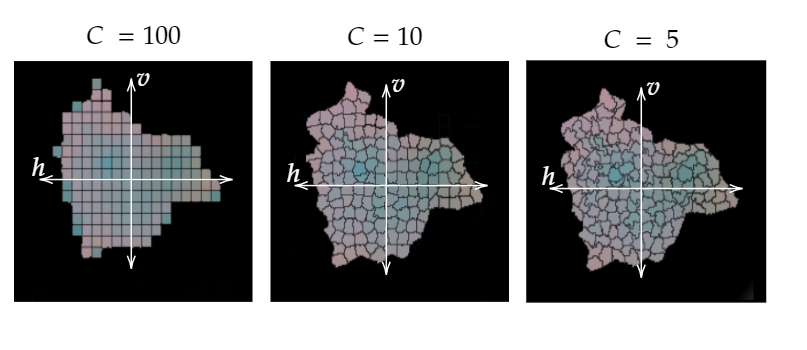
\includegraphics[scale=0.6]{images/superpixels.png}
\caption{This diagram shows the skin lesion split relating to superpixels instead of averaging squares.}
\end{figure}\label{SP}

Each parallel square on the vertical and horizontal axes measures similarity using a three-dimensional Euclidean distance in the LAB colour space. For example, the perceivable difference of colour to the human eye is a three-dimensional Euclidean distance of 6\cite{Myridis2014a}. Using similar logic, a value of 20 is the threshold, where any value over that amount is considered asymmetrical in colour. Next, each square is compared with its closest parallel square (relating to the line through the centre defined by the bi-fold) and removed from an array after being compared. The next improvement is to generate a unique threshold for the significance of each square. For example, using superpixels with the compactness of 10 has an accuracy of 61\% with the PH$^2$ dataset compared to the original 59.5\%. This approach demonstrates that a flexible border that considers features is more effective than averaging squares.

\begin{figure}
\centering
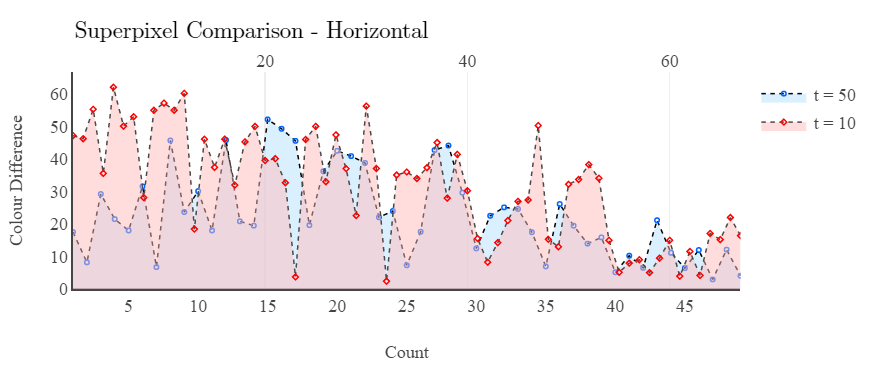
\includegraphics[scale=0.7]{images/superpixel2.png}
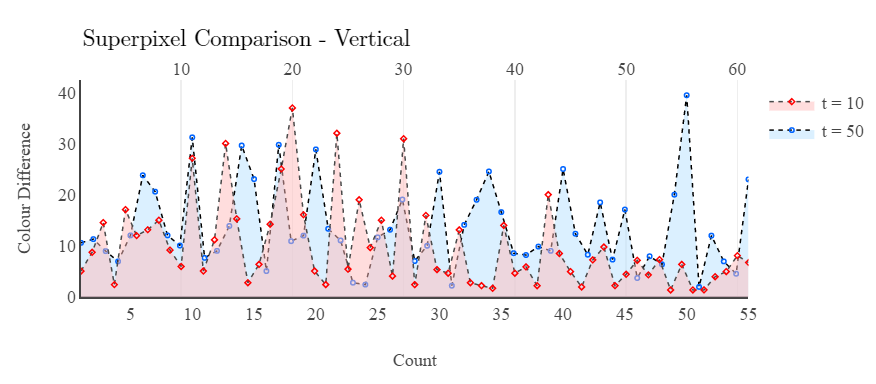
\includegraphics[scale=0.7]{images/superpixel1.png}
\caption{This diagram shows the difference between averaging squares and using superpixels, with the threshold of 10 implying curves and 50 being squares. The horizontal colour difference is improved, making it more likely to be seen asymmetrical. The vertical comparison is roughly the same, except for removing a false positive of 40.}
\end{figure}\label{asy3}

There is a correlation in colour differences between the inner and outer edges because melanoma typically expands outwards, creating an abnormal border. This information specifies that the statistical model accuracy could be improved by increasing the threshold for the outer edges and decreasing it for the inner.

\section{Border Detection Using Zernike Moments, 
Fractal Box-Counting, and Convexity}

\section{A Novel Colour Analysis Approach using Colour Ranges, and SVM}

\section{Dermoscopic structures}

\section{Results}


\section{Conclusion}

% Describe the asymmetry technique and the changes that have been made to it.

%The proposed method has many similarities to Kasmi and Mokrani\cite{Kasmi2016} colour comparison technique, except it is updated to improve accuracy using superpixels, and a Support Vector Machine (SVM).

%The original method uses moments of inertia

%without any flexibility splits areas of interest in half, making comparisons less adequate. Using superpixels allows for a softer border which improves colour separation and accuracy.

%Superpixels are k-means colour extraction techniques designed to separate areas of an image into their associated areas of colour by applying a soft border around the edge.